% Volume III: Probability, Statistics, Information, and Causality
% Continuity note for Chapter 17.
% Previous dependencies: Chapter 13's probability spaces, random variables, joint/conditional distributions, random vectors, covariance, and independence; Chapter 14's Bernoulli, Poisson, Gaussian, multivariate Gaussian, and exponential-family models; Chapter 15's expectation, conditioning, Bayes updates, and decision rules; Chapter 16's LLN, CLT, standard errors, convergence, concentration, and high-dimensional estimation intuition.
% New durable concepts: statistical model, parameter space, data x_{1:n}, likelihood L_n(theta), log-likelihood ell_n(theta), estimator and estimate, MLE, bias, variance, mean squared error, consistency, score, Fisher information, observed information, Cramer-Rao lower bound intuition, standard error from curvature, null and alternative hypotheses, test statistic, p-value, Type I/II error, power, confidence interval, coverage, predictive risk, empirical risk, validation risk, test risk, cross-validation, overfitting, bias-variance tradeoff, AIC/BIC as likelihood-plus-complexity criteria.
% Forward hooks: Chapter 18 reuses likelihood curvature as Fisher geometry and turns uncertainty/distinguishability into entropy, KL divergence, cross-entropy, mutual information, and statistical manifolds; later ML chapters reuse negative log-likelihood, validation/test risk, generalization, calibration, and model comparison; neuroscience chapters reuse firing-rate estimation, neural coding precision, stimulus decoding tests, and held-out predictive likelihood.
% Notation commitments: Data are x_{1:n} or X_1,\ldots,X_n; parameters are theta in Theta; models are p_theta(x) or p_theta(y|x); under iid or conditionally independent observations likelihood is L_n(theta)=prod_i p_theta(x_i); log-likelihood is ell_n(theta)=sum_i log p_theta(x_i); an estimator is hat theta=T(X_1,\ldots,X_n); Fisher information is written mathcal I(theta) to avoid collision with mutual information I(X;Y); predictive loss is c(h(X),Y), not ell, because ell is reserved here for log-likelihood.
% Figure plan: four raster figures under imagegen-figures/ch17-* are referenced: likelihood curve and MLE for 17.1; Fisher curvature and uncertainty for 17.2; a corrected testing/confidence-interval diagram for 17.3; model-selection risk curve for 17.4.
\section{Chapter 17: Statistical Inference and Decision Theory}
\label{ch:statistical-inference-decision-theory}

Chapters 13--15 built probability as a language for uncertainty: random variables, distributions, conditioning, Bayes' theorem, and decisions under incomplete information. Chapter 16 then explained why empirical quantities can become reliable: averages stabilize, standardized errors often become nearly Gaussian, and high-dimensional random objects can concentrate.

Chapter 17 turns those facts into statistical practice. We observe data, choose a model family, estimate unknown quantities, quantify uncertainty, test scientific claims, and select predictive models. The mathematical question is no longer only "what is random?" It is "what should we decide after seeing this random data?"

\paragraph{Chapter problem.}
How do we turn data into defensible estimates, uncertainty statements, hypothesis tests, and model choices while keeping track of sampling variability and predictive consequences?

\paragraph{Section map.}
Section 17.1 introduces likelihood, estimators, maximum likelihood, and the basic bias--variance language of estimation. Section 17.2 uses score functions and Fisher information to connect likelihood curvature with estimator uncertainty. Section 17.3 builds hypothesis tests and confidence intervals from sampling distributions. Section 17.4 frames model selection as a decision problem about predictive risk, not merely training-set fit.

\subsection{17.1 Estimation and likelihood}

\paragraph{Motivating question.}
Given data and a parameterized model \(p_\theta(x)\), which parameter value makes the observed data most plausible, and what exactly is the estimator producing that value?

\paragraph{Beginner setup.}
Statistical inference starts with two ingredients: data and a model family. The data might be coin flips, spike counts, reaction times, image labels, or losses on test examples. A parameterized model family is a collection of possible distributions,
\[
\{p_\theta:\theta\in\Theta\},
\]
where \(\theta\) is the unknown quantity we want to learn.

The smallest nontrivial example is Bernoulli data. Each observation \(X_i\in\{0,1\}\) records failure or success, and the model is
\[
P_\theta(X_i=1)=\theta,\qquad P_\theta(X_i=0)=1-\theta,
\]
with parameter \(\theta\in[0,1]\). If the observed data are \(1,0,1,1,0\), then three successes in five trials suggest \(\theta\) should be near \(3/5\).

The concept solved by likelihood is comparison. It lets us ask, for each candidate \(\theta\), how compatible that candidate is with the data we actually observed. The concept solved by an estimator is action. It gives a rule that turns a random sample into a reported value.

What to keep in mind: a likelihood is a function of the parameter after the data are fixed. It is not, by itself, a probability distribution over \(\theta\). To make a probability distribution over parameters, one needs a prior and Bayes' theorem, as in Chapter 15.

\begin{figure}[htbp]
\centering
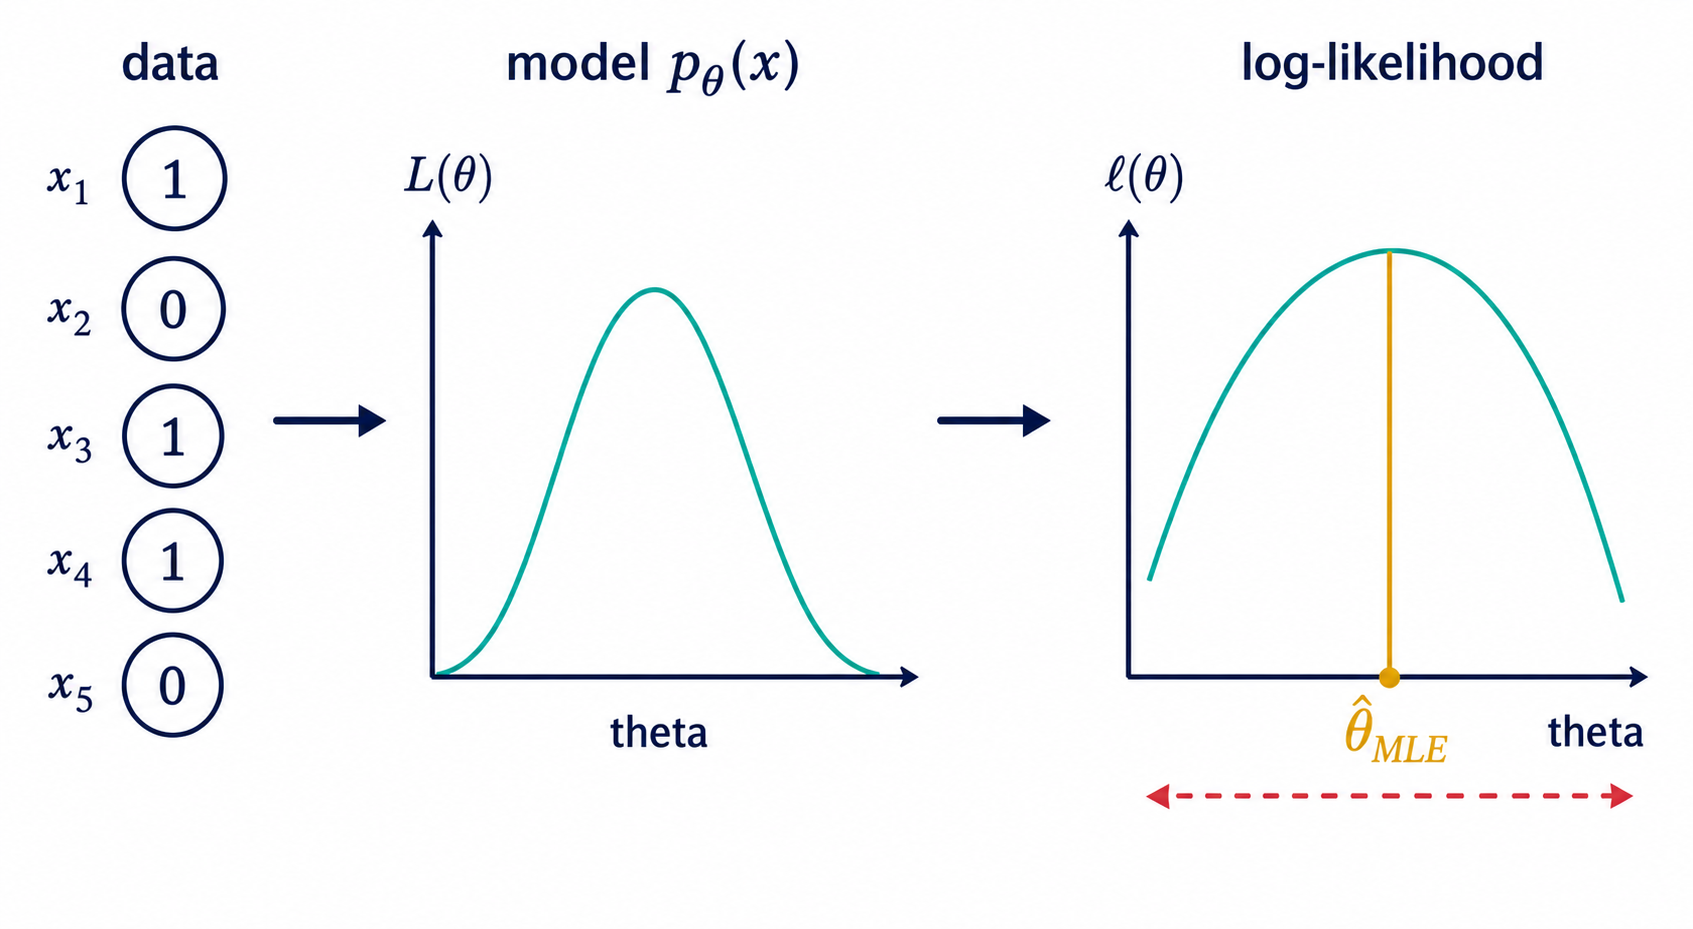
\includegraphics[width=0.98\linewidth]{imagegen-figures/ch17-likelihood-mle.png}
\caption{Likelihood turns observed data into a function of the parameter. For Bernoulli data, candidate values of \(\theta\) assign different probabilities to the same fixed sequence \(x_{1:n}\). The maximum likelihood estimate \(\hat\theta_{\mathrm{MLE}}\) is the parameter value where the likelihood, or equivalently the log-likelihood, is largest.}
\label{fig:ch17-likelihood-mle}
\end{figure}

\paragraph{Formal setup.}
Let \(X_1,\ldots,X_n\) be data drawn from a distribution in a model family \(\{p_\theta:\theta\in\Theta\}\). The observations may be discrete or continuous. In the discrete case \(p_\theta(x)\) is a probability mass function; in the continuous case it is a density with respect to a chosen measure. For the factorized likelihood below, assume the observations are iid under \(p_\theta\), or conditionally independent given their covariates in a conditional model.

For observed data \(x_{1:n}=(x_1,\ldots,x_n)\), the likelihood is
\[
\boxed{
L_n(\theta;x_{1:n})
=\prod_{i=1}^n p_\theta(x_i).
}
\]
The log-likelihood is
\[
\boxed{
\ell_n(\theta;x_{1:n})
=\sum_{i=1}^n \log p_\theta(x_i).
}
\]
The product becomes a sum because independent probabilities multiply and logarithms turn multiplication into addition. This is numerically stable and algebraically useful. If the data are dependent, the likelihood is instead the joint mass or density \(p_\theta(x_{1:n})\), which may not factor into \(\prod_i p_\theta(x_i)\). A time-series model, for example, often factors the joint likelihood into conditional pieces such as \(\prod_i p_\theta(x_i\mid x_{1:i-1})\).

An \emph{estimator} is a function of the random data,
\[
\hat\theta=T(X_1,\ldots,X_n),
\]
and the number obtained after plugging in observed data is an \emph{estimate}. The maximum likelihood estimator is
\[
\boxed{
\hat\theta_{\mathrm{MLE}}
\in
\operatorname{argmax}_{\theta\in\Theta}\ell_n(\theta;X_{1:n}).
}
\]
Because \(\hat\theta\) is a random variable, it has sampling properties. Its bias is
\[
\operatorname{Bias}_\theta(\hat\theta)
=\mathbb E_\theta[\hat\theta]-\theta,
\]
its variance is \(\operatorname{Var}_\theta(\hat\theta)\), and for scalar \(\theta\) its mean squared error is
\[
\operatorname{MSE}_\theta(\hat\theta)
=\mathbb E_\theta[(\hat\theta-\theta)^2]
=\operatorname{Var}_\theta(\hat\theta)+\operatorname{Bias}_\theta(\hat\theta)^2.
\]
An estimator is consistent if \(\hat\theta\to\theta\) in probability under repeated sampling from the true parameter.

\paragraph{Core intuition.}
Figure~\ref{fig:ch17-likelihood-mle} shows the central geometry. The data are fixed on the left. Each possible \(\theta\) says how surprising those data would be. Plotting that compatibility as \(\theta\) varies produces a curve. The MLE is the peak of that curve.

Likelihood is not the same as a probability of the parameter. The expression \(p_\theta(x_{1:n})\) means "probability or density of the data if the parameter were \(\theta\)." Once \(x_{1:n}\) is fixed, \(L_n(\theta)\) is just a nonnegative function of \(\theta\). It need not integrate to one over \(\Theta\).

A second misconception is to treat an estimate as nonrandom. Before data are collected, \(\hat\theta\) is a random variable because it is a function of random observations. After data are collected, it becomes the reported value. This distinction is why Chapter 16 matters: repeated samples would produce repeated estimates, and their variability can be studied.

This section uses Chapter 14's model families and Chapter 16's estimator variability. It prepares Fisher information in Section 17.2, tests and intervals in Section 17.3, and the negative-log-likelihood losses used for predictive modeling in Section 17.4.

\paragraph{Main derivation: Bernoulli maximum likelihood.}
Suppose \(X_1,\ldots,X_n\) are iid Bernoulli\((\theta)\), with the closed parameter space \(\theta\in[0,1]\). We first derive the interior maximum for \(\theta\in(0,1)\). If \(s=\sum_{i=1}^n x_i\), then
\[
L_n(\theta)
=\prod_{i=1}^n \theta^{x_i}(1-\theta)^{1-x_i}
=\theta^s(1-\theta)^{n-s}.
\]
The log-likelihood is
\[
\ell_n(\theta)=s\log\theta+(n-s)\log(1-\theta).
\]
Differentiate:
\[
\frac{d}{d\theta}\ell_n(\theta)
=\frac{s}{\theta}-\frac{n-s}{1-\theta}.
\]
Set the derivative equal to zero:
\[
\frac{s}{\theta}=\frac{n-s}{1-\theta}
\quad\Longleftrightarrow\quad
s(1-\theta)=(n-s)\theta
\quad\Longleftrightarrow\quad
s=n\theta.
\]
Thus
\[
\boxed{\hat\theta_{\mathrm{MLE}}=\frac{s}{n}=\bar X_n.}
\]
The second derivative is
\[
\frac{d^2}{d\theta^2}\ell_n(\theta)
=-\frac{s}{\theta^2}-\frac{n-s}{(1-\theta)^2}<0
\]
when \(0<s<n\), so the critical point is a maximum. The mechanism is simple: the value of \(\theta\) that best explains the observed fraction of successes is the observed fraction itself.

The boundary cases are part of the same closed-space answer. If \(s=0\), then \(L_n(\theta)=(1-\theta)^n\), which is maximized at \(\theta=0\). If \(s=n\), then \(L_n(\theta)=\theta^n\), which is maximized at \(\theta=1\). Therefore the boxed formula \(\hat\theta_{\mathrm{MLE}}=s/n\) holds for all \(s=0,\ldots,n\) on \([0,1]\), with the all-failure and all-success samples landing at the boundary.

The estimator \(\bar X_n\) is unbiased because \(\mathbb E_\theta[\bar X_n]=\theta\), and its variance is
\[
\operatorname{Var}_\theta(\bar X_n)=\frac{\theta(1-\theta)}{n}.
\]
By the law of large numbers, \(\bar X_n\to\theta\) in probability, so the Bernoulli MLE is consistent.

\paragraph{Worked examples.}
\emph{Small numerical example.}
For data \(x_{1:5}=(1,0,1,1,0)\), we have \(s=3\) and \(n=5\). The Bernoulli likelihood is
\[
L_5(\theta)=\theta^3(1-\theta)^2.
\]
The MLE is
\[
\hat\theta_{\mathrm{MLE}}=\frac{3}{5}=0.6.
\]
At \(\theta=0.6\), the likelihood is \(0.6^3(0.4)^2=0.03456\). At \(\theta=0.5\), the likelihood is \(0.5^5=0.03125\). The difference is not huge for five observations, which is exactly why small-sample estimates are uncertain.

\emph{Symbolic Gaussian example.}
Suppose \(X_i\sim\mathcal N(\mu,\sigma^2)\) with known \(\sigma^2\) and unknown \(\mu\). Up to constants not depending on \(\mu\),
\[
\ell_n(\mu)
=-\frac{1}{2\sigma^2}\sum_{i=1}^n (x_i-\mu)^2.
\]
Maximizing this log-likelihood is the same as minimizing \(\sum_i(x_i-\mu)^2\). The best \(\mu\) is the sample mean \(\bar x\). This connects likelihood to least squares from Chapter 5: Gaussian noise turns squared error into negative log-likelihood.

\emph{Neuroscience example.}
If spike counts \(X_i\) in repeated trials are modeled as iid Poisson\((\lambda)\), then
\[
p_\lambda(x_i)=e^{-\lambda}\frac{\lambda^{x_i}}{x_i!}.
\]
The log-likelihood, ignoring constants that do not depend on \(\lambda\), is
\[
\ell_n(\lambda)=-n\lambda+\left(\sum_{i=1}^n x_i\right)\log\lambda.
\]
Differentiating gives \(-n+\sum_i x_i/\lambda=0\), so
\[
\hat\lambda_{\mathrm{MLE}}=\bar x.
\]
The estimated firing rate in the analysis window is the average spike count across trials.

\emph{Machine-learning example.}
For a probabilistic classifier \(p_\theta(y\mid x)\), the conditional log-likelihood of labeled data \((x_i,y_i)\) is
\[
\ell_n(\theta)=\sum_{i=1}^n \log p_\theta(y_i\mid x_i).
\]
Training by minimizing cross-entropy is maximum likelihood in this conditional model, because the training loss is the negative log-likelihood
\[
-\ell_n(\theta)=-\sum_{i=1}^n \log p_\theta(y_i\mid x_i).
\]
The parameter \(\theta\) may contain millions of neural-network weights, but the inference principle is the same as in the Bernoulli example.

\paragraph{ML/DL/neuroscience connections.}
In machine learning, the model \(p_\theta(y\mid x)\) maps inputs to predictive distributions, \(\theta\) is the vector of learned weights, and the estimator is the training algorithm that maps a dataset to fitted weights. In deep learning, negative log-likelihood becomes cross-entropy for classifiers or squared error for Gaussian regression. In neuroscience, \(p_\theta(r\mid s)\) may be a response model for neural activity \(r\) given stimulus \(s\); likelihood compares candidate tuning parameters, gain parameters, or latent states by how well they explain observed spikes.

\paragraph{Exercises.}
\begin{enumerate}[label=\textbf{17.1.\arabic*.}, leftmargin=*]
\item \textbf{Mechanical.} For Bernoulli data \(x_{1:8}=(1,1,0,1,0,0,1,1)\), write the likelihood \(L_8(\theta)\), the log-likelihood \(\ell_8(\theta)\), and the MLE \(\hat\theta_{\mathrm{MLE}}\).
\item \textbf{Proof or derivation.} Derive the MLE for the Poisson mean \(\lambda\) from iid counts \(x_1,\ldots,x_n\), and state where the assumption \(\lambda>0\) enters.
\item \textbf{Numerical/computational.} Evaluate the Bernoulli log-likelihood for the data in the first exercise at \(\theta=0.25,0.50,0.75\). Which value is largest, and how does it compare with the exact MLE?
\item \textbf{Interpretation.} Explain the difference between an estimator and an estimate in the context of fitting a neural firing-rate model from repeated trials.
\item \textbf{Debug the misconception.} A student says, "The likelihood \(L(\theta)\) is the probability that \(\theta\) is true." Correct the statement without using Bayesian priors.
\end{enumerate}

\subsection{17.2 Fisher information and uncertainty}

\paragraph{Motivating question.}
How does the shape of the likelihood curve tell us how uncertain an estimator should be?

\paragraph{Beginner setup.}
Two datasets can have MLEs at the same parameter value but very different uncertainty. A sharply peaked likelihood says that nearby parameter values explain the data much worse. A flat likelihood says that many nearby values explain the data almost equally well.

Fisher information measures this sensitivity. In one dimension, it is the expected squared slope of the log-likelihood contribution from one observation. Equivalently, under regularity conditions, it is the expected curvature of the negative log-likelihood. High information means the distribution changes rapidly as \(\theta\) changes; low information means the data are relatively insensitive to \(\theta\).

The smallest useful example is a Gaussian mean. If \(X\sim\mathcal N(\mu,\sigma^2)\) and \(\sigma^2\) is known, then a small \(\sigma^2\) makes the mean easy to estimate: observations cluster tightly around \(\mu\). A large \(\sigma^2\) makes the same mean harder to estimate. Fisher information makes that statement exact.

What to keep in mind: information here is not entropy and not mutual information. To avoid notation collision with Chapter 18's mutual information \(I(X;Y)\), this chapter writes Fisher information as \(\mathcal I(\theta)\).

\begin{figure}[htbp]
\centering
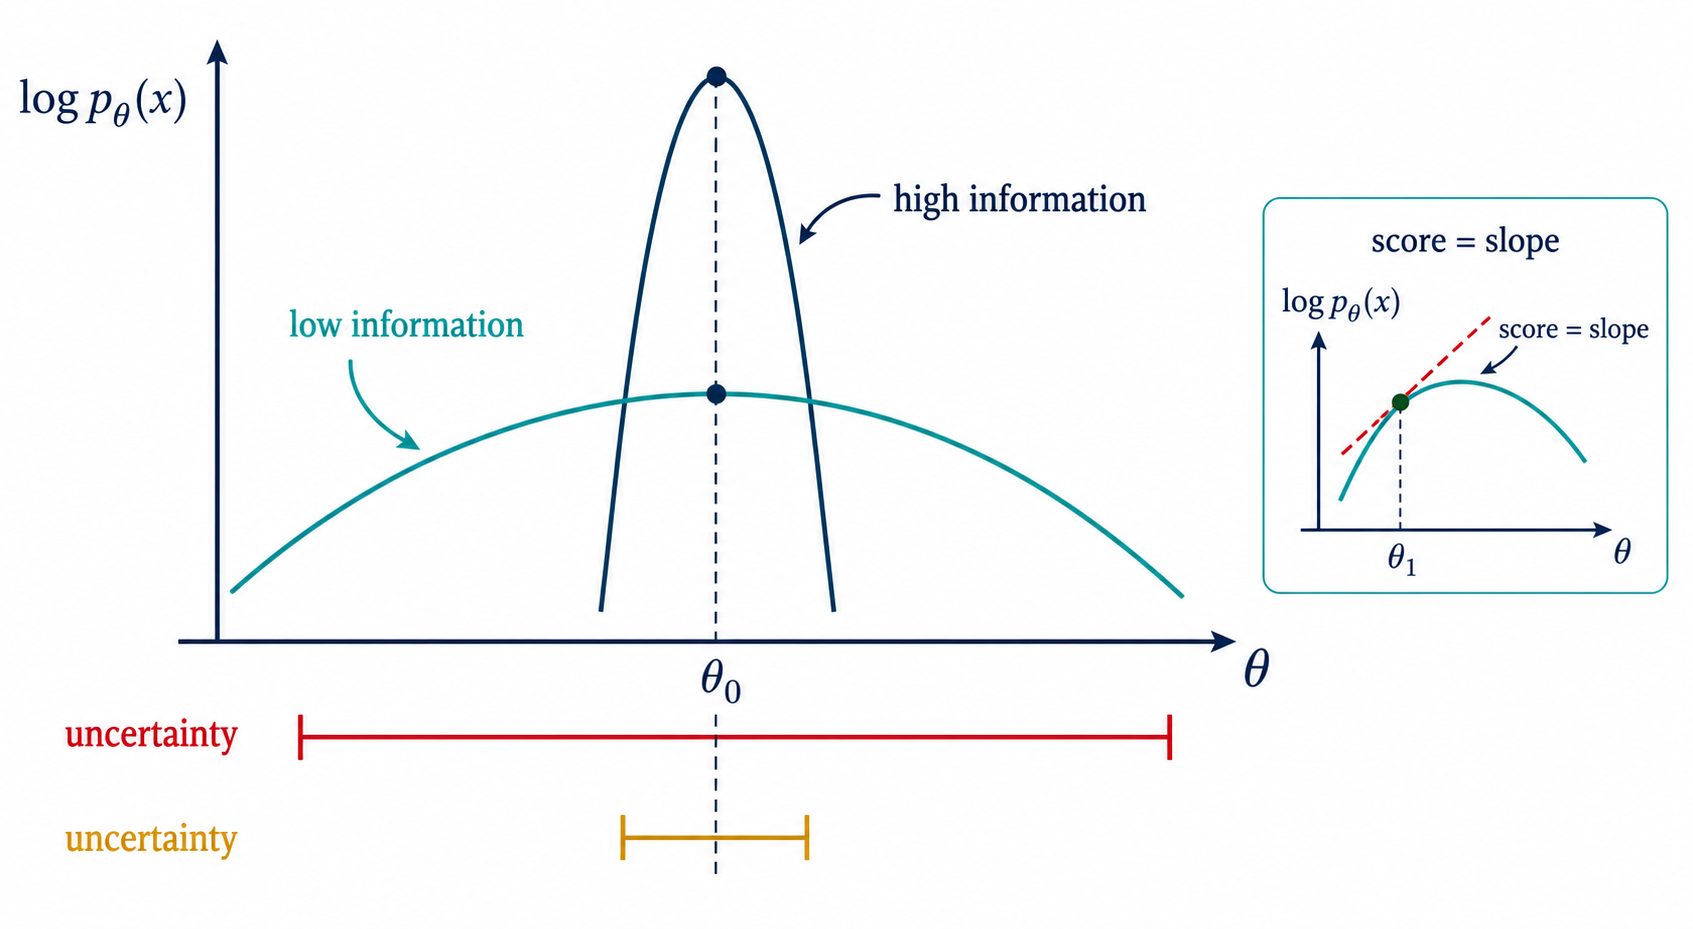
\includegraphics[width=0.98\linewidth]{imagegen-figures/ch17-fisher-curvature-uncertainty.png}
\caption{Fisher information is local sensitivity of the model to the parameter. A steep, sharply curved log-likelihood near the true parameter corresponds to high information and narrow uncertainty. A shallow curve corresponds to low information and wide uncertainty. The score is the slope of the single-observation log density as the parameter changes.}
\label{fig:ch17-fisher-curvature}
\end{figure}

\paragraph{Formal setup.}
Let \(X\sim p_\theta(x)\), where \(\theta\in\Theta\subseteq\mathbb R\). The score for one observation is
\[
\boxed{
s_\theta(X)=\frac{\partial}{\partial\theta}\log p_\theta(X).
}
\]
Under standard regularity conditions that allow differentiating under the integral sign,
\[
\mathbb E_\theta[s_\theta(X)]=0.
\]
The Fisher information in one observation is
\[
\boxed{
\mathcal I_1(\theta)
=\mathbb E_\theta[s_\theta(X)^2].
}
\]
Equivalently, again under regularity conditions,
\[
\boxed{
\mathcal I_1(\theta)
=-\mathbb E_\theta\!\left[
\frac{\partial^2}{\partial\theta^2}\log p_\theta(X)
\right].
}
\]
For iid data \(X_1,\ldots,X_n\), scores add:
\[
s_{n,\theta}(X_{1:n})
=\frac{\partial}{\partial\theta}\ell_n(\theta;X_{1:n})
=\sum_{i=1}^n s_\theta(X_i),
\]
so information adds:
\[
\boxed{\mathcal I_n(\theta)=n\mathcal I_1(\theta).}
\]
For vector parameters \(\theta\in\mathbb R^d\), the score is a gradient and Fisher information is the matrix
\[
\mathcal I_1(\theta)
=\mathbb E_\theta\!\left[
\nabla_\theta\log p_\theta(X)\,
\nabla_\theta\log p_\theta(X)^\top
\right].
\]

\paragraph{Core intuition.}
Figure~\ref{fig:ch17-fisher-curvature} shows why curvature and uncertainty are inverses of each other. A flat likelihood peak leaves many parameter values plausible, so an estimate can vary widely across repeated samples. A sharp peak pins the parameter down more tightly.

The score is a local diagnostic. If changing \(\theta\) slightly changes \(\log p_\theta(X)\) a lot, then the observed data are sensitive to \(\theta\). The squared score is large. Fisher information averages this sensitivity over data generated from the model itself.

Common misconceptions: Fisher information is not the amount of data in bytes. It is parameter-specific statistical sensitivity. It can depend on the true parameter value. It also depends on the model; misspecifying the model can make Fisher-based uncertainty misleading.

This section reuses Chapter 9's gradients and Hessians, Chapter 10's local quadratic approximations, Chapter 16's standard errors, and Section 17.1's log-likelihood. It prepares Chapter 18's information geometry, where Fisher information becomes a local metric on a statistical manifold.

\paragraph{Main theorem: Cramer--Rao lower bound.}
For a scalar parameter \(\theta\), suppose \(\hat\theta\) is an unbiased estimator of \(\theta\) and the model satisfies the regularity assumptions above. Then
\[
\boxed{
\operatorname{Var}_\theta(\hat\theta)
\geq
\frac{1}{\mathcal I_n(\theta)}.
}
\]
This says that an unbiased estimator cannot have variance smaller than the reciprocal of the information in the sample.

\emph{Proof sketch.}
The score has mean zero:
\[
\mathbb E_\theta[s_{n,\theta}(X_{1:n})]=0.
\]
Unbiasedness means
\[
\mathbb E_\theta[\hat\theta]=\theta.
\]
Differentiate both sides with respect to \(\theta\). Under regularity conditions, differentiating the expectation brings down the score:
\[
\frac{\partial}{\partial\theta}\mathbb E_\theta[\hat\theta]
=
\mathbb E_\theta[\hat\theta\,s_{n,\theta}(X_{1:n})]
=1.
\]
Because the score has mean zero, this is also
\[
\operatorname{Cov}_\theta(\hat\theta,s_{n,\theta})=1.
\]
Cauchy--Schwarz gives
\[
\operatorname{Cov}_\theta(\hat\theta,s_{n,\theta})^2
\leq
\operatorname{Var}_\theta(\hat\theta)\,
\operatorname{Var}_\theta(s_{n,\theta}).
\]
The variance of the score is Fisher information:
\[
\operatorname{Var}_\theta(s_{n,\theta})=\mathcal I_n(\theta).
\]
Therefore
\[
1\leq \operatorname{Var}_\theta(\hat\theta)\mathcal I_n(\theta),
\]
which gives the bound. The mechanism is geometric: if the estimator changes correctly with the parameter, it must be correlated with the score, and that correlation cannot exceed what their variances allow.

\paragraph{Worked examples.}
\emph{Gaussian mean.}
Let \(X\sim\mathcal N(\mu,\sigma^2)\) with known \(\sigma^2\). The log density, ignoring constants, is
\[
\log p_\mu(X)=-\frac{(X-\mu)^2}{2\sigma^2}.
\]
The score is
\[
s_\mu(X)=\frac{\partial}{\partial\mu}\log p_\mu(X)=\frac{X-\mu}{\sigma^2}.
\]
Thus
\[
\mathcal I_1(\mu)
=\mathbb E_\mu\!\left[\frac{(X-\mu)^2}{\sigma^4}\right]
=\frac{\sigma^2}{\sigma^4}
=\frac{1}{\sigma^2}.
\]
For \(n\) iid observations, \(\mathcal I_n(\mu)=n/\sigma^2\), so the Cramer--Rao bound is
\[
\operatorname{Var}(\hat\mu)\geq\frac{\sigma^2}{n}.
\]
The sample mean attains this bound, since \(\operatorname{Var}(\bar X)=\sigma^2/n\).

\emph{Bernoulli parameter.}
For \(X\sim\mathrm{Bernoulli}(\theta)\),
\[
\log p_\theta(X)=X\log\theta+(1-X)\log(1-\theta).
\]
The score is
\[
s_\theta(X)=\frac{X}{\theta}-\frac{1-X}{1-\theta}
=\frac{X-\theta}{\theta(1-\theta)}.
\]
Since \(\operatorname{Var}_\theta(X)=\theta(1-\theta)\),
\[
\mathcal I_1(\theta)
=\frac{1}{\theta^2(1-\theta)^2}\operatorname{Var}_\theta(X)
=\frac{1}{\theta(1-\theta)}.
\]
For \(n\) observations, information is \(n/(\theta(1-\theta))\), and the reciprocal information is \(\theta(1-\theta)/n\), matching the variance of \(\bar X\).

\emph{Neural coding example.}
Suppose a neuron's spike count \(R\) in a time window is modeled as Poisson with stimulus-dependent rate \(\lambda(\theta)\), where \(\theta\) is stimulus orientation. For a Poisson model,
\[
\mathcal I_1(\theta)
=\frac{(\lambda'(\theta))^2}{\lambda(\theta)}.
\]
The numerator says that firing rate must change with the stimulus to carry information. The denominator says that high variability in counts reduces precision. For independent neurons, Fisher informations add under the model assumptions, so a population can estimate orientation more precisely when many neurons have steep tuning curves near that orientation.

\emph{Deep-learning example.}
For a probabilistic neural network \(p_\theta(y\mid x)\), the Fisher information matrix averages outer products of score gradients:
\[
\mathcal I(\theta)
=\mathbb E\!\left[
\nabla_\theta\log p_\theta(Y\mid X)
\nabla_\theta\log p_\theta(Y\mid X)^\top
\right].
\]
Natural-gradient methods precondition ordinary gradients by an approximation to \(\mathcal I(\theta)^{-1}\). The mathematical object is the same Fisher matrix: it rescales parameter updates according to how much the predictive distribution changes in each direction.

\paragraph{ML/DL/neuroscience connections.}
In statistical learning, Fisher information describes local identifiability of parameters. In deep learning, it appears in natural gradients, second-order optimization approximations, continual-learning penalties, and uncertainty estimates near fitted parameters. In neuroscience, Fisher information maps neural response distributions \(p_\theta(r)\) to stimulus precision: the parameter \(\theta\) becomes stimulus value, the random variable \(R\) becomes the neural response, and \(\mathcal I(\theta)^{-1}\) sets a lower bound on decoding variance under the model.

\paragraph{Exercises.}
\begin{enumerate}[label=\textbf{17.2.\arabic*.}, leftmargin=*]
\item \textbf{Mechanical.} For \(X\sim\mathcal N(\mu,4)\) with known variance, compute the score \(s_\mu(X)\), the one-sample Fisher information, and the \(n\)-sample Cramer--Rao lower bound for unbiased estimators of \(\mu\).
\item \textbf{Proof or derivation.} Starting from \(p_\theta(x)=\theta^x(1-\theta)^{1-x}\), derive the Bernoulli score and Fisher information \(\mathcal I_1(\theta)=1/(\theta(1-\theta))\).
\item \textbf{Numerical/computational.} For Bernoulli data with \(n=200\) and true \(\theta=0.25\), compute the approximate standard error \(1/\sqrt{\mathcal I_n(\theta)}\). Compare it with \(\sqrt{\theta(1-\theta)/n}\).
\item \textbf{Interpretation.} In a neural orientation-coding model, what happens to Fisher information near a stimulus value where the tuning curve is flat, so \(\lambda'(\theta)\approx0\)? Explain in terms of decoding precision.
\item \textbf{Debug the misconception.} A student says, "High Fisher information means the dataset has high entropy." Correct the statement by distinguishing entropy from parameter sensitivity.
\end{enumerate}

\subsection{17.3 Hypothesis testing and confidence intervals}

\paragraph{Motivating question.}
How can we decide whether data provide evidence against a proposed parameter value, and how can we report a range of parameter values compatible with the data-generating process?

\paragraph{Beginner setup.}
Hypothesis testing starts with a claim called the null hypothesis. For example, a coin is fair, a treatment has no effect, two neural firing rates are equal, or a classifier performs at chance. A test statistic compresses the data into one number whose behavior is known or approximated when the null is true.

A confidence interval starts from the same sampling-variability problem but reports a range instead of a yes/no decision. A \(95\%\) confidence interval is produced by a procedure that covers the true parameter in \(95\%\) of repeated samples, under the assumptions used to build it.

The smallest useful example is a sample proportion. If \(n=100\) trials produce \(\hat p=0.61\), is that enough evidence against \(H_0:p=0.5\)? The answer depends not only on the difference \(0.61-0.5\), but also on the standard error of \(\hat p\).

What to keep in mind: tests and intervals are about procedures under repeated sampling. A p-value is not the probability that the null is true. A frequentist \(95\%\) confidence interval does not mean the fixed true parameter has \(95\%\) probability of lying in this particular realized interval.

\begin{figure}[htbp]
\centering
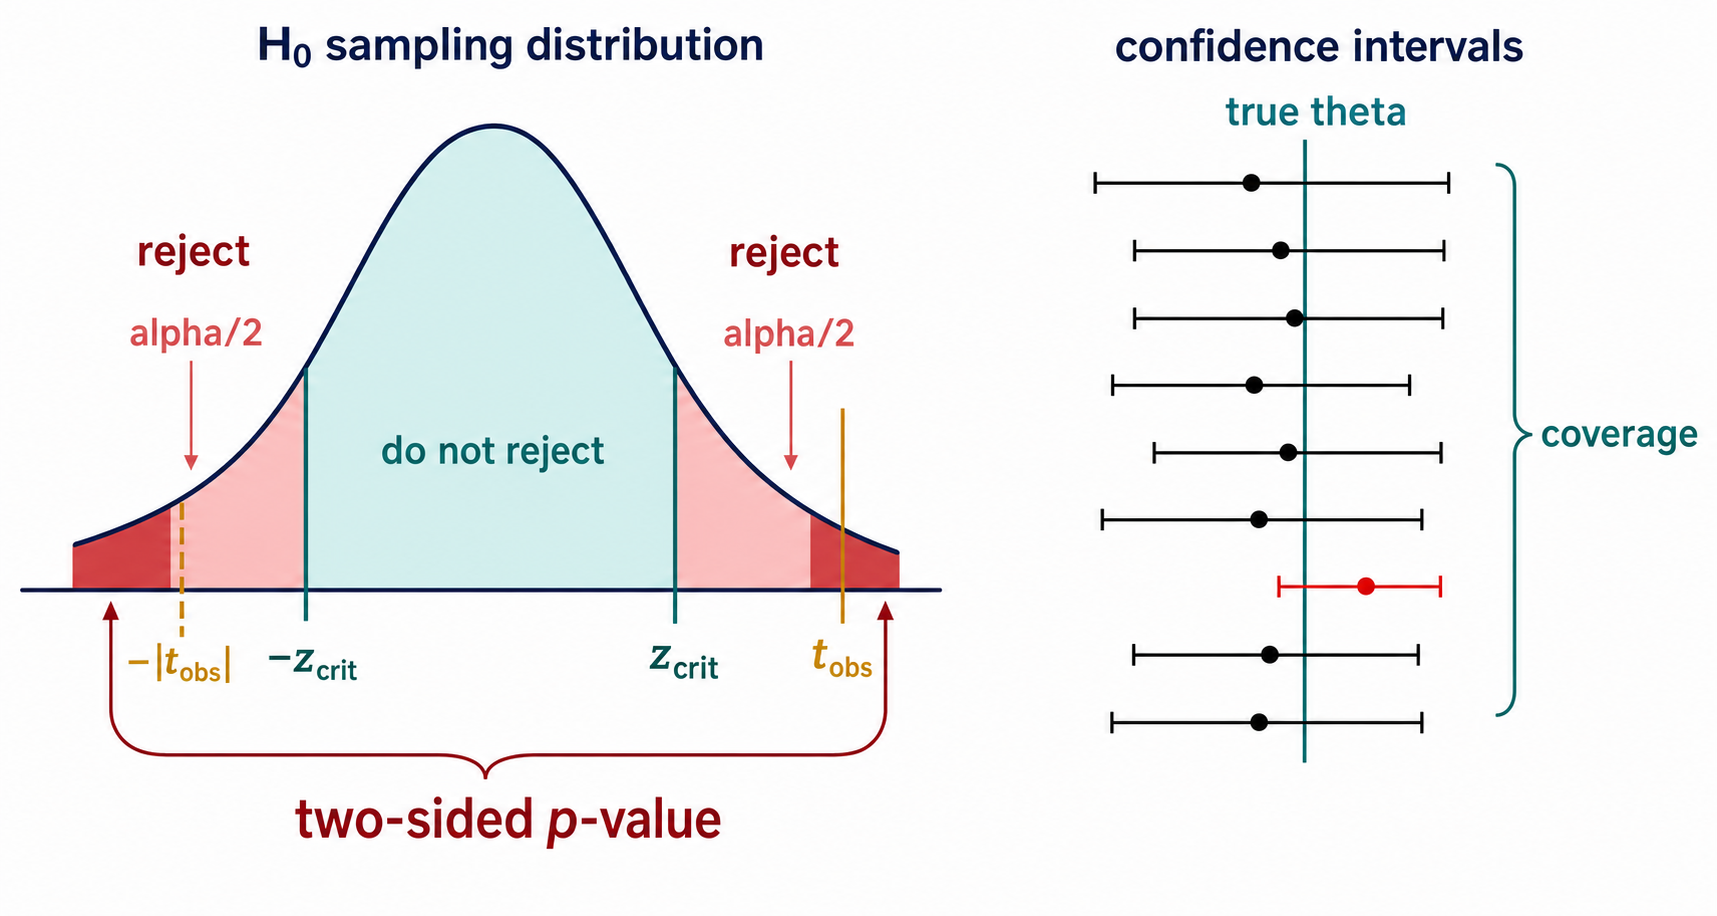
\includegraphics[width=0.98\linewidth]{imagegen-figures/ch17-testing-ci.png}
\caption{Testing and confidence intervals are two views of sampling distributions. A hypothesis test compares the observed statistic with its null distribution and rejects in prechosen tail regions. For a two-sided test, the p-value is the sum of both null tails beyond \(\pm |t_{\mathrm{obs}}|\), not the whole prechosen \(\alpha/2\) rejection region. A confidence-interval procedure produces random intervals that cover the fixed true parameter at the advertised long-run rate.}
\label{fig:ch17-testing-ci}
\end{figure}

\paragraph{Formal setup.}
Let data \(X_{1:n}\) come from a model with parameter \(\theta\). A null hypothesis \(H_0\) is a restricted claim, such as
\[
H_0:\theta=\theta_0.
\]
An alternative hypothesis \(H_1\) describes departures of interest, such as
\[
H_1:\theta\neq\theta_0
\quad\text{or}\quad
H_1:\theta>\theta_0.
\]
A test statistic is a function \(T(X_{1:n})\). Its null distribution is the distribution of \(T\) assuming \(H_0\) is true. A rejection rule with significance level \(\alpha\) satisfies
\[
\boxed{
P_{H_0}(\text{reject }H_0)\leq\alpha.
}
\]
This probability is the Type I error rate. The Type II error rate at an alternative parameter value is
\[
\beta(\theta)=P_\theta(\text{fail to reject }H_0),
\]
and the power is \(1-\beta(\theta)\).

A p-value is the null probability of seeing a test statistic at least as extreme as the observed statistic, according to the chosen direction of extremeness. For a two-sided approximately normal statistic \(Z\),
\[
\boxed{
p\text{-value}=2P(Z_{\mathrm{null}}\geq |z_{\mathrm{obs}}|)
}
\]
where \(Z_{\mathrm{null}}\sim\mathcal N(0,1)\).

A \(1-\alpha\) confidence interval is a random set \(C(X_{1:n})\) such that
\[
\boxed{
P_\theta(\theta\in C(X_{1:n}))\approx 1-\alpha.
}
\]
The approximation comes from asymptotic normality, large-sample standard errors, or model-specific exact calculations.

\paragraph{Core intuition.}
Figure~\ref{fig:ch17-testing-ci} separates the two procedures. In the testing panel, the null distribution is the world we would expect if \(H_0\) were true. The observed statistic lands somewhere on that reference curve. If it falls in a prespecified tail region, the data are unusual under the null, so we reject.

In the interval panel, repeated samples produce different centers and different intervals. Most intervals cover the true parameter, but some miss. The coverage statement belongs to the procedure over repeated samples, not to a hidden random motion of the true parameter.

Common misconceptions cause many scientific errors. A small p-value does not measure effect size; a tiny effect can be significant with huge \(n\). Failing to reject \(H_0\) does not prove \(H_0\); it may mean low power. A \(95\%\) interval does not guarantee that \(95\%\) of future observations fall in the interval; it is about the parameter, not new data values.

This section uses Chapter 16's CLT and standard errors, Section 17.1's estimators, and Section 17.2's curvature-based uncertainty. It prepares model comparison and predictive evaluation, where rejection of a simple null is often less informative than estimating predictive gains.

\paragraph{Main derivation: Wald tests and confidence intervals.}
Suppose an estimator is approximately normal:
\[
\hat\theta\approx \mathcal N(\theta,\operatorname{se}(\hat\theta)^2).
\]
Under \(H_0:\theta=\theta_0\), the standardized statistic
\[
\boxed{
Z=\frac{\hat\theta-\theta_0}{\operatorname{se}(\hat\theta)}
}
\]
is approximately \(\mathcal N(0,1)\). A two-sided level-\(\alpha\) Wald test rejects \(H_0\) when
\[
|Z|>z_{1-\alpha/2},
\]
where \(z_{1-\alpha/2}\) is the corresponding standard-normal quantile.

The associated approximate \(1-\alpha\) confidence interval is
\[
\boxed{
\hat\theta\pm z_{1-\alpha/2}\operatorname{se}(\hat\theta).
}
\]
Why does this work? If
\[
\frac{\hat\theta-\theta}{\operatorname{se}(\hat\theta)}
\approx \mathcal N(0,1),
\]
then with probability about \(1-\alpha\),
\[
-z_{1-\alpha/2}
\leq
\frac{\hat\theta-\theta}{\operatorname{se}(\hat\theta)}
\leq
z_{1-\alpha/2}.
\]
Multiplying by \(\operatorname{se}(\hat\theta)\) and rearranging gives
\[
\hat\theta-z_{1-\alpha/2}\operatorname{se}(\hat\theta)
\leq
\theta
\leq
\hat\theta+z_{1-\alpha/2}\operatorname{se}(\hat\theta).
\]
Thus the interval is an algebraic inversion of the sampling statement. Tests and intervals are not separate tricks; they are two forms of the same approximate normal comparison.

\paragraph{Worked examples.}
\emph{Bernoulli proportion test.}
Suppose \(n=100\) binary trials produce \(61\) successes, so \(\hat p=0.61\). Test
\[
H_0:p=0.5
\quad\text{against}\quad
H_1:p\neq0.5.
\]
Under \(H_0\), the standard error of \(\hat p\) is
\[
\sqrt{\frac{0.5(1-0.5)}{100}}=0.05.
\]
The test statistic is
\[
Z=\frac{0.61-0.50}{0.05}=2.2.
\]
The two-sided p-value is approximately
\[
2P(N(0,1)\geq2.2)\approx0.028.
\]
At level \(0.05\), this rejects the fair-coin null.

\emph{Confidence interval for the same proportion.}
Using the estimated standard error
\[
\sqrt{\frac{0.61(0.39)}{100}}\approx0.049,
\]
an approximate \(95\%\) confidence interval is
\[
0.61\pm1.96(0.049)
\approx
[0.514,0.706].
\]
The interval does not contain \(0.5\), consistent with the two-sided level-\(0.05\) test.

\emph{Neuroscience example.}
Suppose a neuron is recorded under two stimuli. Across repeated trials, the estimated mean spike-count difference is
\[
\hat\Delta=\bar X_A-\bar X_B=3.0
\]
spikes in the analysis window, with standard error \(1.2\). Testing \(H_0:\Delta=0\) gives
\[
Z=\frac{3.0}{1.2}=2.5,
\]
with a two-sided p-value about \(0.012\). A \(95\%\) interval is
\[
3.0\pm1.96(1.2)=[0.65,5.35].
\]
The objects map directly: \(\Delta\) is the stimulus effect on mean response, \(\hat\Delta\) is the observed difference, and the standard error summarizes trial-to-trial variability.

\emph{Machine-learning example.}
To compare two classifiers on the same \(n=1000\) test examples, define \(D_i=1\) if model A is correct and model B is wrong, \(D_i=-1\) if B is correct and A is wrong, and \(D_i=0\) otherwise. The mean \(\bar D\) estimates the accuracy advantage of A over B on this paired test set. A standard-error calculation for \(\bar D\) supports a confidence interval for the accuracy difference. This is stronger than comparing two raw accuracies as if they came from unrelated test sets.

\paragraph{ML/DL/neuroscience connections.}
In ML, tests and intervals quantify uncertainty in accuracy, AUC, calibration error, loss differences, and ablation effects. The parameter might be a population risk difference rather than a model weight. In neuroscience, tests compare firing rates, decoding accuracies, tuning-curve slopes, or latent-state effects across conditions. The mathematical objects map cleanly: the estimator is the measured effect, the null is a scientific no-effect claim, the test statistic standardizes by uncertainty, and the interval reports a range of compatible effect sizes.

\paragraph{Exercises.}
\begin{enumerate}[label=\textbf{17.3.\arabic*.}, leftmargin=*]
\item \textbf{Mechanical.} A sample proportion is \(\hat p=0.54\) from \(n=400\) trials. Under \(H_0:p=0.5\), compute the approximate standard error and the \(Z\)-statistic.
\item \textbf{Proof or derivation.} Starting from \((\hat\theta-\theta)/\operatorname{se}(\hat\theta)\approx N(0,1)\), derive the approximate \(95\%\) confidence interval \(\hat\theta\pm1.96\operatorname{se}(\hat\theta)\).
\item \textbf{Numerical/computational.} For a neural firing-rate difference \(\hat\Delta=1.8\) with standard error \(0.75\), compute the \(Z\)-statistic and an approximate \(95\%\) confidence interval.
\item \textbf{Interpretation.} A study fails to reject \(H_0:\Delta=0\) at level \(0.05\), but the confidence interval is \([-4.2,4.8]\) spikes. What does this say about evidence, uncertainty, and practical effect size?
\item \textbf{Debug the misconception.} A student says, "A p-value of \(0.03\) means there is a \(3\%\) chance the null hypothesis is true." Correct the statement using the definition of a p-value.
\end{enumerate}

\subsection{17.4 Model selection and predictive risk}

\paragraph{Motivating question.}
When several models fit the training data, how should we choose the one that will make the best future predictions?

\paragraph{Beginner setup.}
Estimation finds parameters inside a model. Model selection chooses among models, feature sets, architectures, regularization strengths, or complexity levels. The key quantity is not training error by itself. The key quantity is predictive risk: expected loss on new data from the same population.

The smallest useful example is polynomial regression. A degree-0 model may underfit because it cannot follow the signal. A degree-20 model may fit the training points extremely well but behave badly on new points. A middle-complexity model can have lower predictive risk even if it does not minimize training error.

The problem solved by validation and test sets is honest evaluation. Training data are used to fit parameters. Validation data are used to choose among models or hyperparameters. Test data are held back for final performance reporting.

What to keep in mind: a model is a decision. It commits us to future predictions and future losses. Model selection is therefore decision theory applied to predictors.

\begin{figure}[htbp]
\centering
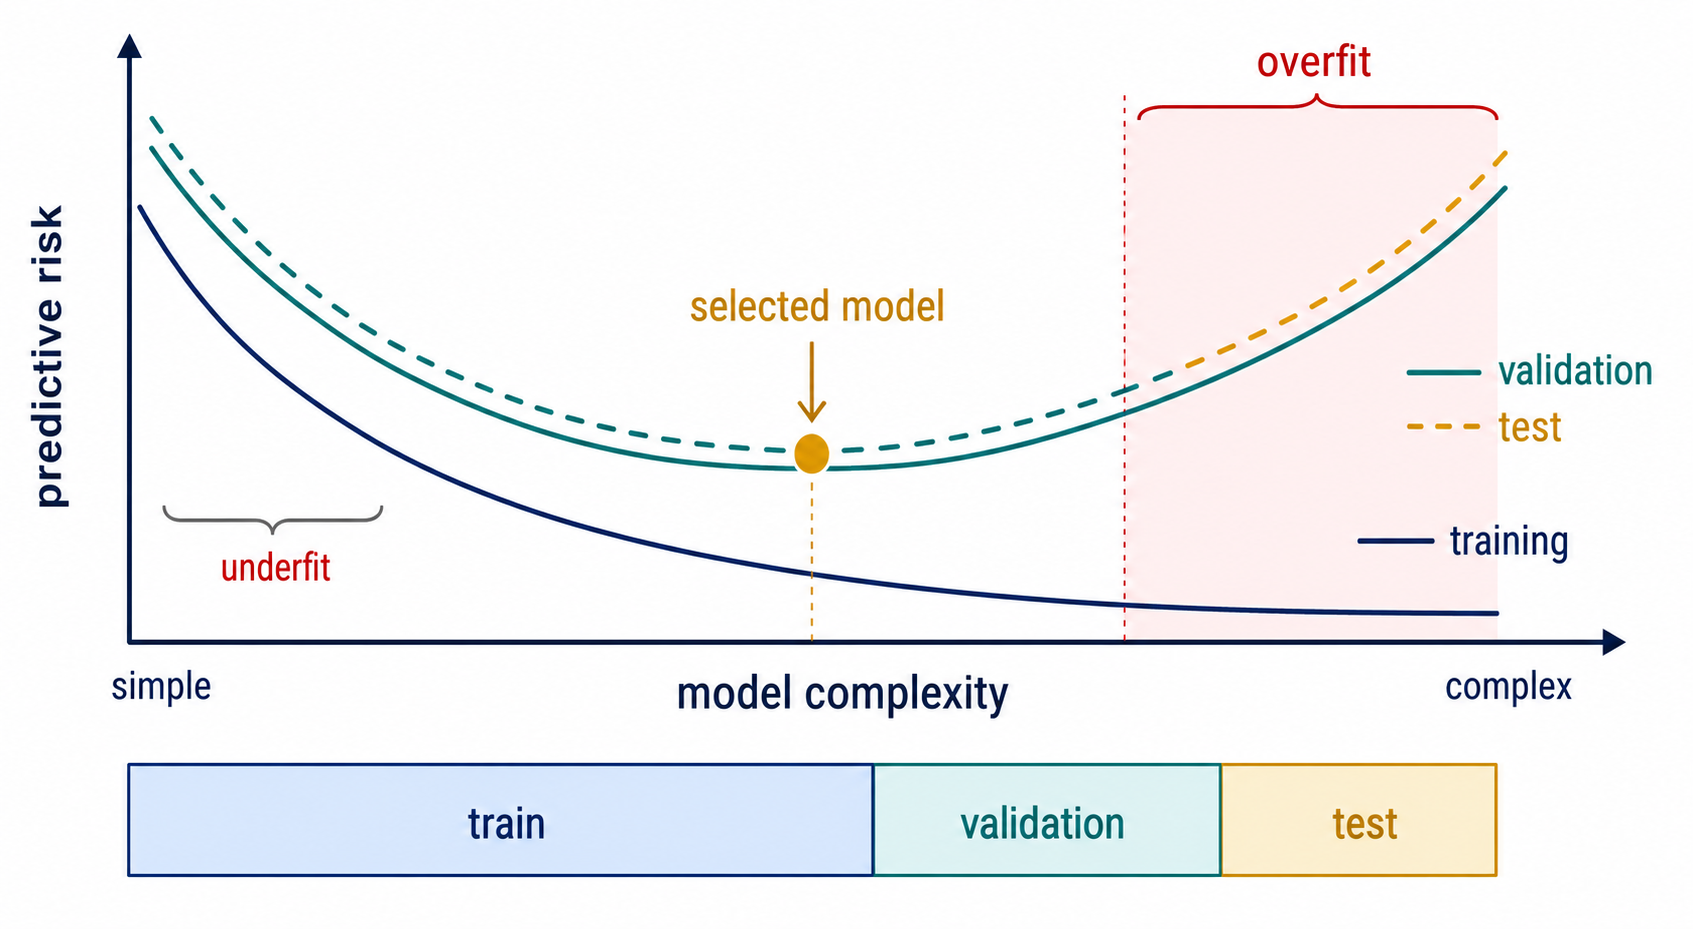
\includegraphics[width=0.98\linewidth]{imagegen-figures/ch17-model-selection-risk.png}
\caption{Model selection should track predictive risk, not only training fit. Training risk often decreases with model complexity, while validation and test risk can be U-shaped. The selected model is near the minimum validation risk; very simple models underfit, and overly complex models can overfit.}
\label{fig:ch17-model-selection-risk}
\end{figure}

\paragraph{Formal setup.}
Let \((X,Y)\sim P\) be a new input-output pair from the target population. A fitted prediction rule is \(h:\mathcal X\to\mathcal Y\), and a loss function is
\[
c(h(X),Y)\geq0.
\]
The predictive risk is
\[
\boxed{
R(h)=\mathbb E[c(h(X),Y)].
}
\]
For training data \(D_{\mathrm{train}}=\{(x_i,y_i)\}_{i=1}^n\), empirical training risk is
\[
\hat R_{\mathrm{train}}(h)
=\frac{1}{n}\sum_{i=1}^n c(h(x_i),y_i).
\]
If a fitted model \(\hat h_m\) comes from model class or hyperparameter choice \(m\), and validation data \(D_{\mathrm{val}}\) are independent of the training data, the validation risk estimate is
\[
\boxed{
\hat R_{\mathrm{val}}(m)
=\frac{1}{|D_{\mathrm{val}}|}
\sum_{(x_i,y_i)\in D_{\mathrm{val}}}
c(\hat h_m(x_i),y_i).
}
\]
The validation-selected model is
\[
\hat m\in\operatorname{argmin}_m \hat R_{\mathrm{val}}(m).
\]
A final test risk estimate uses data not used for fitting or selection.

For likelihood-based models, a common predictive loss is negative log-likelihood:
\[
c(p_\theta(\cdot\mid X),Y)=-\log p_\theta(Y\mid X).
\]
Information criteria approximate out-of-sample predictive performance using fitted likelihood plus a complexity penalty. In a \(k\)-parameter model,
\[
\mathrm{AIC}=2k-2\ell_n(\hat\theta),
\qquad
\mathrm{BIC}=k\log n-2\ell_n(\hat\theta).
\]
Lower values are preferred, but these criteria rely on assumptions; validation remains the more direct predictive check when sufficient data are available.

\paragraph{Core intuition.}
Figure~\ref{fig:ch17-model-selection-risk} shows the typical risk pattern. Training risk decreases as models become more flexible because the model can adapt to the training sample. Predictive risk may first decrease and then increase. On the left, models underfit: their approximation bias is too large. On the right, models overfit: they adapt to noise, idiosyncrasies, or finite-sample artifacts.

The key beginner mistake is to choose the model with the smallest training error. That often selects the most flexible model, not the best predictor. A second mistake is to repeatedly inspect the test set during model development; this turns the test set into a validation set and makes final performance estimates too optimistic.

This section reuses Chapter 15's decision-theoretic risk, Chapter 16's concentration of empirical averages, and Section 17.1's negative log-likelihood. It prepares later machine-learning generalization theory and Chapter 18's cross-entropy/KL view of predictive distributions.

\paragraph{Main derivation: validation risk estimates predictive risk.}
Fix a model choice \(m\) and suppose \(\hat h_m\) was trained without using the validation set. Conditional on the trained predictor \(\hat h_m\), each validation loss
\[
C_i=c(\hat h_m(X_i),Y_i)
\]
is an iid draw from the future-loss distribution of that fixed predictor. Therefore
\[
\mathbb E[\hat R_{\mathrm{val}}(m)\mid \hat h_m]
=
\mathbb E[c(\hat h_m(X),Y)\mid \hat h_m]
=R(\hat h_m).
\]
So validation risk is an unbiased estimate of predictive risk for a fixed trained model.

The variance also shrinks with validation size:
\[
\operatorname{Var}(\hat R_{\mathrm{val}}(m)\mid\hat h_m)
=
\frac{\operatorname{Var}(C_i\mid\hat h_m)}{|D_{\mathrm{val}}|}.
\]
This is Chapter 16's averaging principle applied to future losses.

There is one subtlety. If we choose the minimum over many validation estimates, the winning estimate is biased downward because it was selected partly for being low by chance. Cross-validation, nested validation, and final untouched test sets are practical ways to manage this selection optimism.

\paragraph{Worked examples.}
\emph{Polynomial-degree selection.}
Suppose polynomial degrees \(0,1,2,3,4\) give validation mean squared errors
\[
1.42,\quad 0.83,\quad 0.51,\quad 0.55,\quad 0.78.
\]
Training error might keep decreasing through degree \(4\), but validation risk is lowest at degree \(2\). The decision rule selects degree \(2\) because it gives the best estimate of future squared error among the candidates.

\emph{Simple bias--variance calculation.}
For squared error at a fixed input \(x\), suppose
\[
Y=f^\star(x)+\varepsilon,\qquad \mathbb E[\varepsilon]=0,\qquad \operatorname{Var}(\varepsilon)=\sigma^2.
\]
The fitted predictor \(\hat h\) is random because it depends on the training sample. The future noise term \(\varepsilon\) is from an independent future observation at the same input and is independent of the training sample. With expectations taken over both sources of randomness,
\[
\mathbb E[(\hat h(x)-Y)^2]
=
\left(\mathbb E[\hat h(x)]-f^\star(x)\right)^2
+
\operatorname{Var}(\hat h(x))
+
\sigma^2.
\]
The three terms are squared bias, estimator variance, and irreducible noise. Increasing model complexity often reduces bias but increases variance. Predictive risk balances these terms.

\emph{Neuroscience model comparison.}
Suppose two models predict held-out spike counts from stimulus history: a linear-nonlinear Poisson model and a recurrent latent-state model. For trial \(i\), the predictive loss can be
\[
-\log p_{\hat\theta}(r_i\mid s_i,\text{history}_i).
\]
The model with lower held-out negative log-likelihood assigns higher probability to the observed neural responses. This comparison is about predictive risk on held-out trials, not about which model has more parameters or better training likelihood.

\emph{Deep-learning example.}
When choosing a neural-network architecture or regularization strength, training loss alone usually favors larger models. A validation set estimates the future loss of each trained candidate. The final test set estimates the predictive risk of the selected workflow. The object \(h\) is the trained network, \(c\) is cross-entropy or another task loss, and \(R(h)\) is expected loss on new data.

\paragraph{ML/DL/neuroscience connections.}
In ML, predictive risk is the population objective behind generalization. Empirical training risk is what optimization directly reduces; validation risk is what model selection uses; test risk is what final reporting should estimate. In deep learning, the candidates may differ by architecture, optimizer, data augmentation, early-stopping time, or regularization. In neuroscience, candidates may be encoding models, decoding models, latent dynamical systems, or competing scientific hypotheses. The same mapping holds: predictors are fitted models, losses are scientific or predictive penalties, and risk is expected future error.

\paragraph{Exercises.}
\begin{enumerate}[label=\textbf{17.4.\arabic*.}, leftmargin=*]
\item \textbf{Mechanical.} A classifier uses regularization strengths \(10,1,0.1,0.01\). Their validation losses are \(0.62,0.48,0.44,0.47\), respectively. Which strength is selected by validation risk?
\item \textbf{Proof or derivation.} Show that, for a fixed trained predictor \(\hat h\) independent of the validation set, \(\mathbb E[\hat R_{\mathrm{val}}(\hat h)\mid\hat h]=R(\hat h)\).
\item \textbf{Numerical/computational.} For validation losses \(C_i\) with sample standard deviation \(0.8\) across \(m=256\) validation examples, estimate the standard error of the validation risk mean.
\item \textbf{Interpretation.} A model has lower training loss than a competitor but higher validation loss. Explain what this suggests about overfitting and predictive risk.
\item \textbf{Debug the misconception.} A student says, "The test set can be used after every modeling change because it is not used for gradient updates." Correct the statement using the distinction between validation and final test risk.
\end{enumerate}

\paragraph{Closing bridge.}
Chapter 17 turned probability into statistical decisions. Likelihood made parameters comparable; Fisher information connected local model sensitivity to uncertainty; tests and intervals converted sampling distributions into evidence statements; predictive risk made model choice a decision about future loss. Chapter 18 now asks how to measure uncertainty and distinguishability themselves. Entropy, KL divergence, cross-entropy, mutual information, and Fisher geometry will give a common language for coding, inference, representation learning, and neural information.

\clearpage
